\section{Implementation}
\subsubsection{Ziel}
\begin{itemize}
	\item Code-Qulität verbessern
	\item Coding-Geschwindigkeit erhöhen
	\item Besseres Teamwork
	\item Entwickler unterstützen
\end{itemize}
\subsection{Coding Guidlines}
\subsubsection{Build errors}
\begin{itemize}
	\item Der Code sollte ohne Warnungen kompilieren
	\item Sicherstellen, dass man Warnungen und Fehlermeldungen versteht
	\item Code umschreiben, um Fehler und Warnungen zu eliminieren, aber Lesbarkeit erhalten
\end{itemize}
\subsubsection{Automated build system}
\begin{itemize}
	\item Full: Das ganze System 
	\item Incremental: Nur neubauen, was sich verändert hat
	\item Für Zielarchitektur bauen
	\item Debug und Veröffentlichung
\end{itemize}
\subsubsection{Version control}
$\bold{Verwendung}$:
\begin{itemize}
	\item Verschiedene Teiles einer Datei parallel ändern
	\item Aktuelle Änderungen mergen
	\item Versionen und Merging automatisieren
	\item Bugs und Änderungen nachvollziehen 
\end{itemize}
$\bold{Erhaltung}$:
\begin{itemize}
	\item Häufiges Pushen, besonders nach erfolgreichen Tests
	\item Niemals fehlerhaften Code Pushen 
\end{itemize}
\subsection{Design Guidelines}
Jede Einheit sollte ein einzige Aufgabe haben, da sie ansonsten schwerer wieder zu verwenden ist, verwirrende Interfaces erzeugt und die Implementation schwieriger wird.
\subsubsection{KISS}
\begin{itemize}
	\item Korrekt ist besser als schnell
	\item Einfach ist besser als komplex
	\item Durchsichtig ist besser als süß
	\item Sicher ist besser als unsicher
\end{itemize}
\subsubsection{Scalability}
\begin{itemize}
	\item Flexible, dynamische Daten anstatt fixen Arrays
	\item Lineare Algorithmen, die lineare Algorithmen aufrufen sind quadratisch
	\item Konstant > logarithmisch > linear
	\item Vermeide Algorithmen, die über linear laufen
	\item Niemals exponentiell, außer nicht anderes möglich
\end{itemize}
\subsection{Coding Style}
\subsubsection{Magic numbers}
\begin{itemize}
	\item Nutze verständliche Namen und Ausdrücke
	\item Vermeide hard-coding Werte
	\item Nutze symbolische Konstanten
	\item Symbolische Konstanten separieren, für leichtere Erhaltung
	\item Die gleichen Werte nicht duplizieren 
\end{itemize}
\subsubsection{Variables}
\begin{itemize}
	\item Deklariere Variablen so lokal wie möglich
	\item Die Lebensspanne einer Variable sollte so kurz wie möglich sein
	\item Lasse Variablen nicht uninitialisiert
	\item Uninitialisierte Varibalen können zu unvorhersehbaren Ergebnissen führen  
\end{itemize}
\subsubsection{Cyclic dependencies}
\begin{itemize}
	\item Entsteht, wenn zwei Module voneinander abhängig sind
	\item Untergraben Modularität
	\item Interdependencies können durch unabhängige abstrakte Klassen aufgelöst werden
	\item Transitive Abhängigkeit entsteht, wenn Klassen indirekt von einander abhängig sind
\end{itemize}
\begin{table}[H]
\caption{Cyclic and transitive dependency}
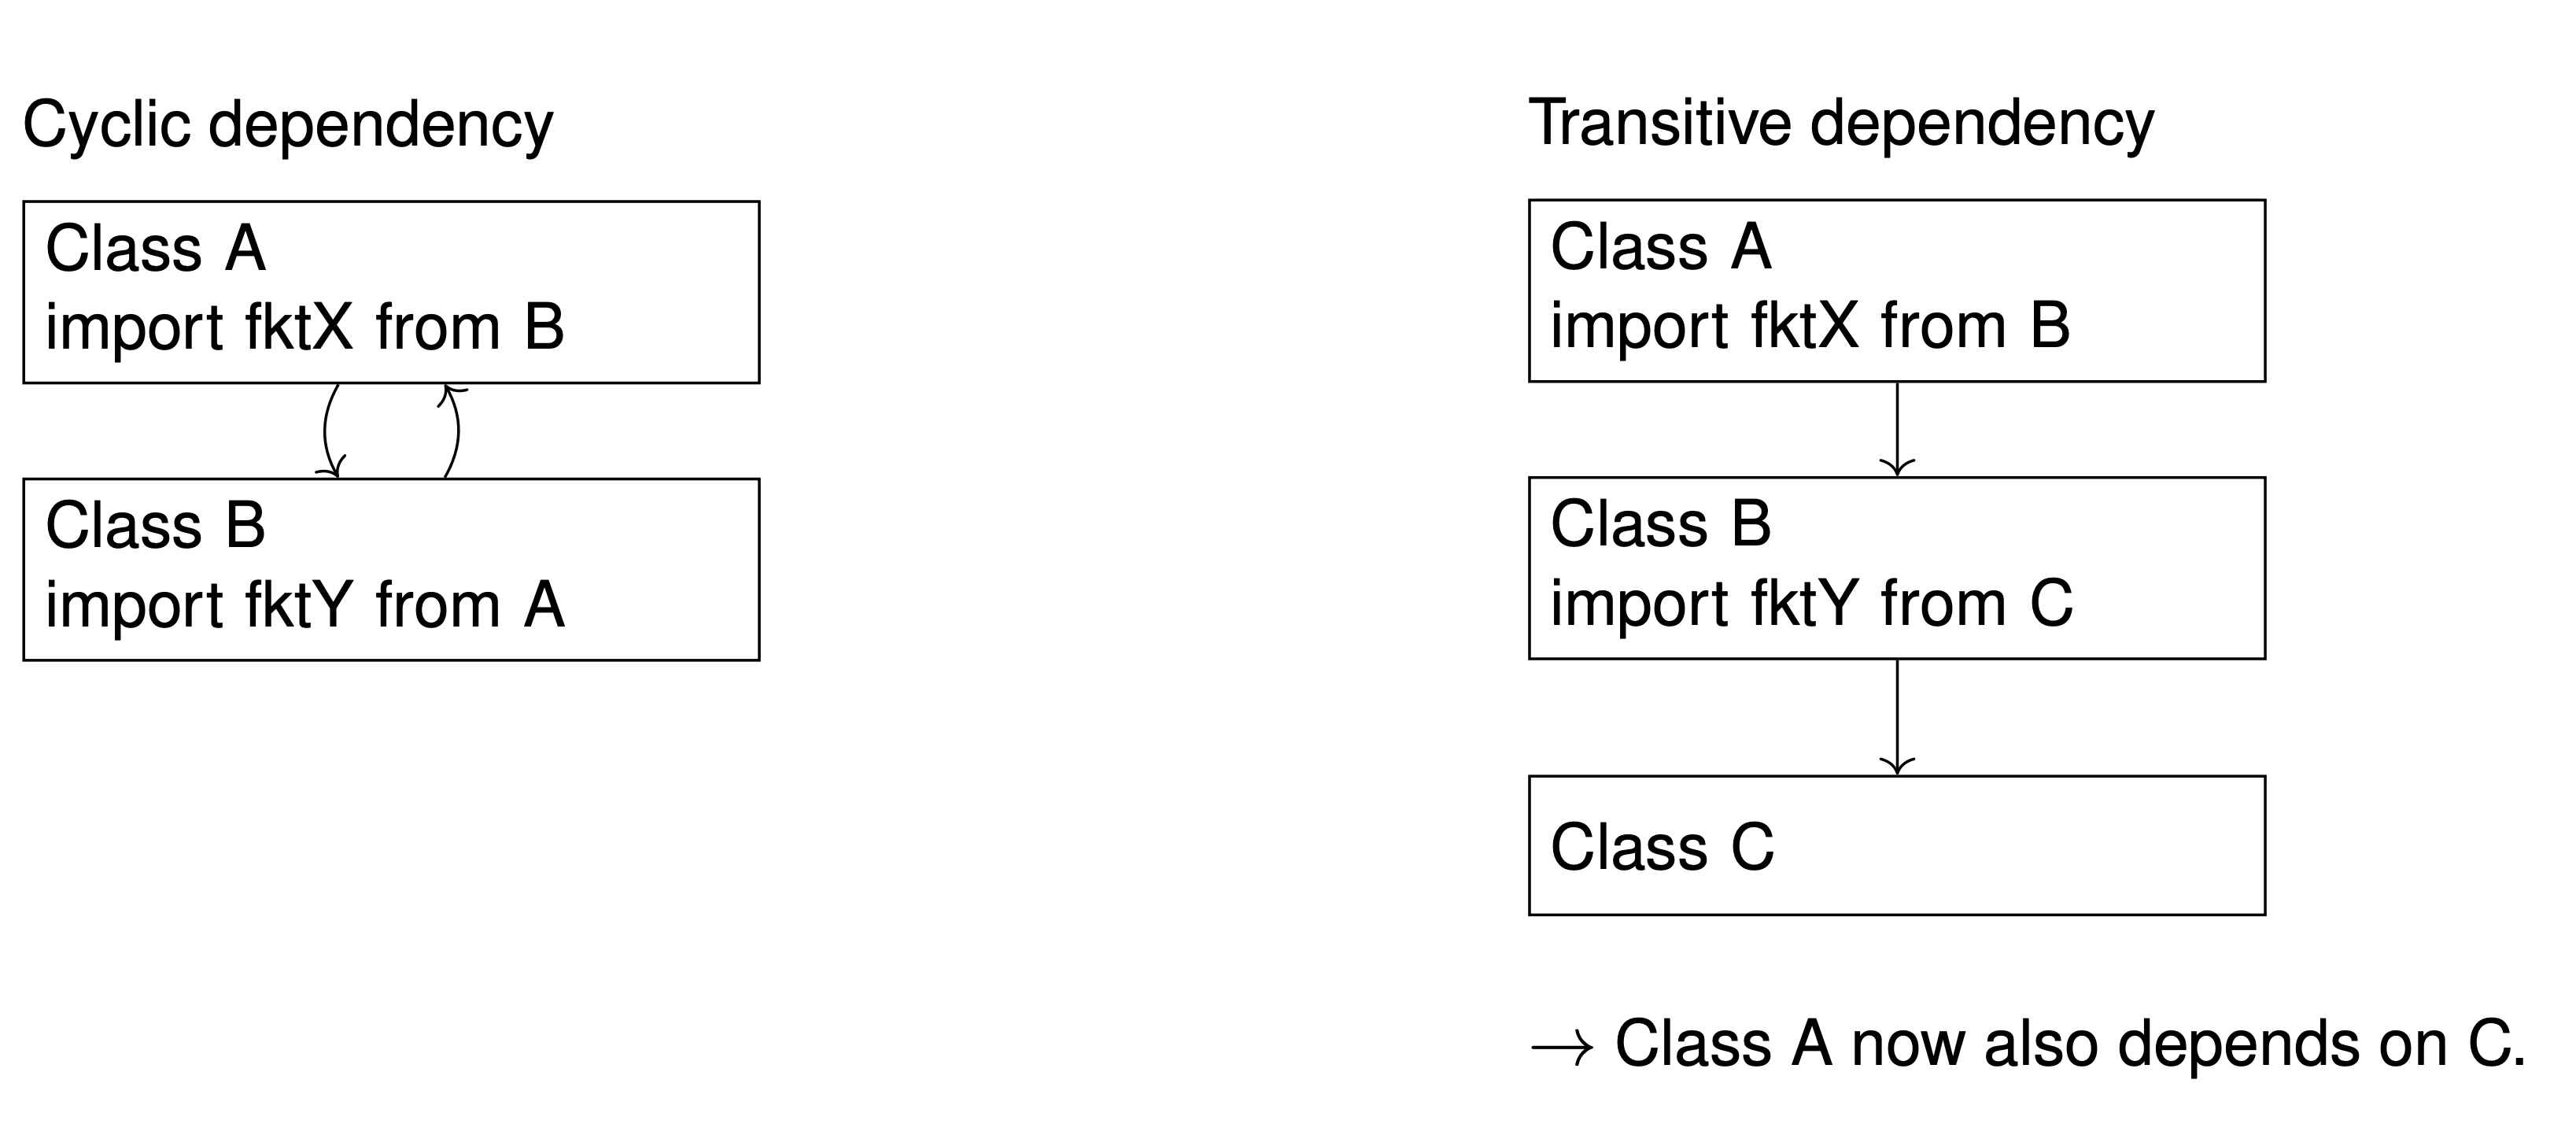
\includegraphics[scale=0.25]{Cyclic_dependency.png}	
\end{table}
\subsubsection{Functions}
\begin{itemize}
	\item Gebe jeder Funktion eine Aufgabe
	\item DRY
	\item Vermeide unnötiges nesting
	\item Verwende Algorithmen anstatt von deep loops
\end{itemize}
\subsubsection{Classes}
$\bold{Typen}$:
\begin{itemize}
	\item $\bold{Value}$ $\bold{class}$: Definiert Objekte, die ihren Wert nach Erzeugung nicht verändern
	\item $\bold{Base}$ $\bold{class}$: Definiert eine Basis, von welcher Kindklassen erben
	\item $\bold{Traits}$ $\bold{class}$: Definiert zusätzliche Traits, die unter Objekte geteilt werden
	\item $\bold{Template}$: Pattern od Code
	\item $\bold{Exception}$ $\bold{class}$: Definiert bestimmte Ausnahmen
\end{itemize}
Verwende minimal classes anstatt komplexen Klassen, Kompositionen anstatt Vererbung
\subsubsection{Memory management}
Vermeide unnötiges kopieren von Variablen und lösche Variablen, wenn möglich nach Gebrauch, um Speicher wieder freizugeben
\subsubsection{Errors and exceptions}
\begin{itemize}
	\item Dokumentiere was der Code tun sollte
	\item Gehe explizit sicher, das der Code die Eigenschaften erfüllt
	\item Entdecke Implementationsfehler
	\item Unterstütze Debugging
\end{itemize}
Eine strikte error handling policy sollte früh im Projekt eingeführt werden
\begin{itemize}
	\item Identifikation  
	\item Wichtigkeit
	\item Erkennung
	\item Meldung
	\item Handhabung
\end{itemize}




